Before talking about the implementation itself, I want to define the main objective of this simple implementation. I want to expose an \textbf{HTTP GET endpoint}, which return a simple \textit{Hello World} string. Unfortunately, that's where the simple stuff ends.\vspace{14pt}\\
First of all, I tried to read \textbf{Apache Openwhisk documentation}\footnote{\url{https://openwhisk.apache.org/documentation.html}} to understand more the Openwhisk environment's setup process.\\
After different attempts to make the \textit{Docker} setup work, I even tried the \textit{Java Standalone} version. Nothing was working the way it was supposed to. I even tried deploying everything on different virtual machines, other than my own machine.\vspace{14pt}\\
I then decided to talk with \textit{Prof. Ciancarini} to get a different point of view of the problem. He suggested reaching out to \textit{Michele Sciabarrà}, the author of the book \textbf{Learning Apache OpenWhisk}\footnote{\url{https://www.oreilly.com/library/view/learning-apache-openwhisk/9781492046158/}}, which runs a company that uses Apache Openwhisk as the backbone of their service. The company is called \textbf{Nuvolaris}\footnote{\url{https://www.nuvolaris.io/}}, and it offers a new serverless approach to Kubernetes.\\
While talking with Sciabarrà, he suggested to use their \textit{spin-off} of Openwhisk, called \textbf{Apache OpenServerless}\footnote{\url{https://openserverless.apache.org/}}, which has a simpler way of deploying the Openwhisk core functionalities.\vspace{14pt}\\
Unfortunately, this process will not be any simpler. I had issues related to this process of deployment too. Reading their documentation, the process was similar to the other one, with less dependencies needed.\\
After some days, during which I tried every possible way of making it work, I tried talking directly with the creators of the Apache OpenServerless software. With their help, I managed to get the system to work, and to finally deploy my \textit{"simple"} implementation.\vspace{14pt}\\
Heartfelt thanks go to \textit{Michele Sciabarrà} and his team, for real-time support while debugging the various problems encountered.\\
Also, a big thank you to the \textbf{ADM team}\footnote{\url{https://students.cs.unibo.it/}} -- especially \textit{Emanuele Grasso}. Thanks to his support, I was provided with a virtual machine that met the requirements of OpenServerless and allowed me to perform all the necessary tests. Their work goes beyond this, providing a very useful service for all students in the Computer Science department and beyond.\vspace{14pt}\\
Let's get back to the implementation.\vspace{14pt}\\
Using the \textit{OpenServerless CLI} (\textbf{ops}), I managed to get everything up and running on the virtual machine. I then wrote a really simple \textbf{Python} script, which returns an \textit{Hello World} message:
\begin{lstlisting}[language=python]
def main(args):
    return {"body": "hello world\n"}
\end{lstlisting}
\vspace{15pt}
Using the \vspace{-5pt}
\begin{center}
    \colorbox{codegray}{\texttt{ops package create test\_dss}}
\end{center} 
command, I created a test package where \textit{actions} can be stored.\\
\begin{center}
    \colorbox{codegray}{\texttt{ops action create test\_dss/greet script.py --web true}}
\end{center} 
is going to create the action related to the Python script. Using the \textit{--web} flag with a value of \textit{true} or \textit{yes} allows an action to be accessible via \textbf{REST} interface without the need for credentials.\vspace{14pt}\\
To get the URL related to the action, the
\begin{center}
    \colorbox{codegray}{\texttt{ops action get test\_dss/greet --url}}
\end{center} 
command is used. This returns the action HTTP endpoint, ready to be called and tested.\vspace{150pt}\\
An example of this whole execution of commands can be:
\begin{center}
    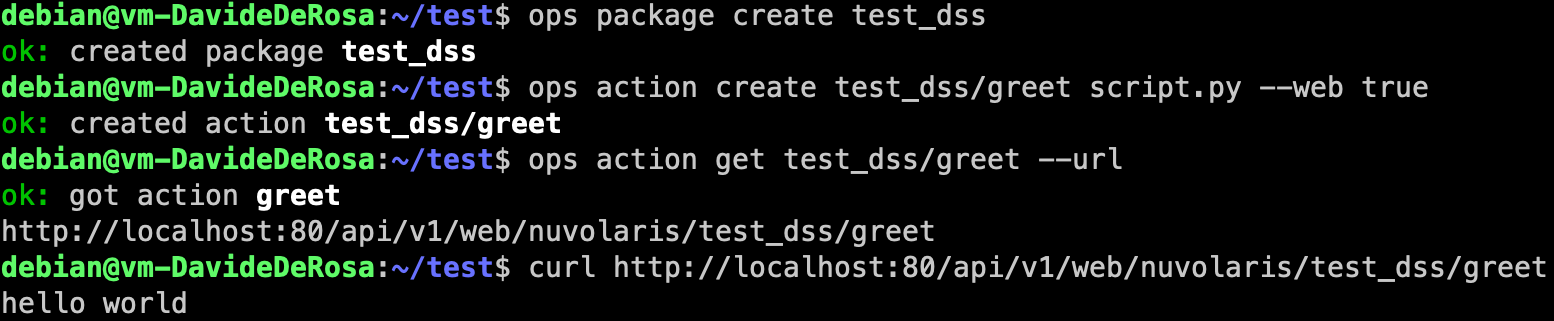
\includegraphics[width=1\textwidth]{img/demo.png}
\end{center}
If you need to update the script, 
\begin{center}
    \colorbox{codegray}{\texttt{ops action update test\_dss/greet script.py --web true}}
\end{center}
is all you need to do.\vspace{14pt}\\
This test shows just the core functionalities of Openwhisk (and OpenServerless). There is a lot more that can be done with this tool. The documentation shows a lot of possible implementations to do, all related to serverless functions.\vspace{14pt}\\
In a possible future study, it would be possible to test Openwhisk performance compared to other Cloud based solution -- like \textit{AWS Lambda} or \textit{Google Cloud Functions}.